\documentclass[../main.tex]{subfiles}
\graphicspath{{\subfix{../images/}}}
\begin{document}

\bigskip\bigskip
\subsection{Inclination Change}

In Section \ref{sec:Mn Manuever}, maneuvers were done at a constant angle to the velocity vector. However, it is more efficient to transfer to the desired orbit directly by finding the vector difference between the old velocity and the desired velocity. To maximize the effect of such a manuever, it should be done at either the ascending or descending node (such that $\Delta j=\Delta i$).

\begin{figure}[H]
    \centering
    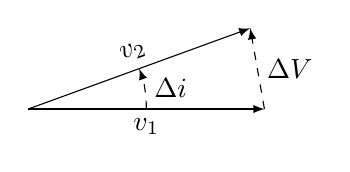
\begin{tikzpicture}[>=latex]
        \def\vel{3}
        \def\dPhi{20}
        \def\arcRad{1.5}

        \draw[->] (0,0) -- +(\dPhi:\vel) node[midway,above,sloped] {$v_2$};
        \draw[->] (0,0) -- +(\vel,0) node[midway,below] {$v_1$};
        \draw[dashed, ->] (\vel,0) -- (\dPhi:\vel) node[midway,right] {$\Delta V$};
        \draw[dashed, ->] (\arcRad,0) arc (0:\dPhi:\arcRad) node[midway, right] {$\Delta i$};
    \end{tikzpicture}
    \caption{Inclination change velocity}\label{fig:dV Triangle Inclination Chage}
\end{figure}

Because the only effect of this maneuver is to change the direction of velocity, $\Delta V$ is the magnitude of the vector difference in the old velocity and the new velocity. Note that, throughout this maneuver, the magnitude of velocity will first decrease and then increase, so there is no net effect on the shape of the orbit in its own plane.

\begin{align*}
    \Delta V & = |\vv{v}_2-\vv{v}_1|                                                    \\
             & = |(v\cos(\Delta i)\hat{m}_v+v\sin(\Delta i)\hat{m}_n)-(v\hat{m}_v)|     \\
             & = |v(\cos(\Delta i)-1)\hat{m}_v+v\sin(\Delta i)\hat{m}_n|                \\
             & = \sqrt{(v(\cos(\Delta i)-1))^2+(v\sin(\Delta i))^2}                     \\
             & = \sqrt{v^2(\cos(\Delta i)-1)^2+v^2\sin^2(\Delta i)}                     \\
             & = v\sqrt{(\cos(\Delta i)-1)^2+\sin^2(\Delta i)}                          \\
             & = v\sqrt{\cos^2(\Delta i)+1-2\cos(\Delta i)+\sin^2(\Delta i)}            \\
             & = v\sqrt{(\cos^2(\Delta i)+\cos^2(\Delta i))+1-2\cos(\Delta i)}          \\
             & = v\sqrt{2-2\cos(\Delta i)}                                              \\
             & = v\sqrt{2(1-\cos(\Delta i))}                                            \\
             & = v\sqrt{2\left(1-\cos\left(2\frac{\Delta i}{2}\right)\right)}           \\
             & = v\sqrt{4\left(\frac{1-\cos\left(2\frac{\Delta i}{2}\right)}{2}\right)} \\
             & = v\sqrt{4\sin^2\left(\frac{\Delta i}{2}\right)}                         \\
\end{align*}

This gives us the $\Delta V$ required for an inclination change maneuver
\begin{equation}
    \Delta V= 2\sin\left(\frac{\Delta i}{2}\right)
\end{equation}

This shows the minimum required $\Delta V$ for an orbital inclination change. If the inclination change occurs at any point other than the ascending or descending node, it will require a greater $\Delta V$ and will also have the effect of chaning the longitude of ascending node $\Omega$ (and therefore moving the ascending and descending nodes). In-plane maneuvers will change neither the inclination nor the longitude of ascending node.

\bigskip\bigskip
\subsection{Hohmann Transfer}\label{sec:Hohmann Transfer}

A Hohmann Transfer is a transfer between two circular orbits from radius $r_1$ to radius $r_2$. The transfer is done via an elliptical orbit, and takes two burns. The first burn puts the orbit into an elliptical orbit in which the periapsis is the lower orbit, and the apoapsis is the higher orbit. The second burn transfers from the elliptic orbit into the final circular orbit.

\begin{figure}[H]
    \centering
    \def\Rone{0.75}
    \def\Rtwo{2.5}
    \def\transSMA{\fpeval{(\Rone+\Rtwo)/2}}
    \def\ctrX{\fpeval{\Rone-\transSMA}}
    \def\trE{\fpeval{\Rtwo/\transSMA - 1}}
    \def\transSmA{\fpeval{\transSMA*sqrt(1-(\trE)^2)}}
    \def\dV{1.25}
    \definecolor{purp}{rgb}{.8,0,.8}
    \begin{tikzpicture}[>=latex]
        \draw[thin, dotted, blue] (0,0) ellipse ({\Rone} and {\Rone});
        \draw[blue, thick,>-] (-\Rone,0) arc (180:360:{\Rone} and {\Rone}) node[right] {$r_1$};


        \draw[thin, dotted, purp] (\ctrX,0) ellipse ({\transSMA} and {\transSmA});
        \draw[purp, thick] (\Rone,0) arc (0:180:{\transSMA} and {\transSmA});

        \draw[thin, dotted,red] (0,0) ellipse ({\Rtwo} and {\Rtwo});
        \draw[red, thick,->] (-\Rtwo,0) arc (180:360:{\Rtwo} and {\Rtwo}) node[right] {$r_2$};;

        \filldraw[lightgray] (0,0) circle (2pt);

        \draw[->] (\Rone,0)--+(0,\dV) node[above] {$\Delta v_1$};
        \draw[->] (-\Rtwo,0)--+(0,-\dV) node[below] {$\Delta v_2$};

    \end{tikzpicture}
    \begin{tikzpicture}[>=latex]
        \draw[->] (\Rone,0)--+(0,-\dV) node[below] {$\Delta v_1$};
        \draw[->] (-\Rtwo,0)--+(0,\dV) node[above] {$\Delta v_2$};

        \draw[thin, dotted, red] (0,0) ellipse ({\Rone} and {\Rone});
        \draw[red, thick,->] (\Rone,0) arc (0:180:{\Rone} and {\Rone}) node[left] {$r_2$};


        \draw[thin, dotted, purp] (\ctrX,0) ellipse ({\transSMA} and {\transSmA});
        \draw[purp, thick] (-\Rtwo,0) arc (180:360:{\transSMA} and {\transSmA});

        \draw[thin, dotted,blue] (0,0) ellipse ({\Rtwo} and {\Rtwo});
        \draw[blue, thick,>-] (\Rtwo,0) arc (0:180:{\Rtwo} and {\Rtwo}) node[left] {$r_1$};;

        \filldraw[lightgray] (0,0) circle (2pt);

    \end{tikzpicture}
    \caption{A Hohmann Transfer from a low orbit to a high orbit (left) and from a high orbit to a lower one (right)}\label{fig:Hohmann Transfer}
\end{figure}

Because both burns are along the velocity vector, $\Delta V=\Delta v_1+\Delta v_2$. $a_1=r_1=r_\text{pe,tr}$ will refer to the semi-major axis of the smaller orbit, with $a_2=r_2=r_\text{ap,tr}$ being the semi-major axis of the larger orbit. The semi-major axis of the transfer orbit is $a_\text{tr}=\frac{1}{2}(r_1+r_2)$. $v_1$ and $v_2$ refer to the circular orbit velocities in the original and new orbit. The below calculations assume a transfer from a low orbit into a higher one.

\begin{align*}
    \Delta V & = \Delta v_1+\Delta v_2                                                                                                                                                                                                           \\
             & = (v_\text{pe,tr}-v_1)+(v_2-v_\text{ap,tr})                                                                                                                                                                                       \\
             & = \left(\sqrt{\frac{2\mu}{r_\text{pe,tr}}-\frac{\mu}{a_\text{tr}}}-\sqrt{\frac{2\mu}{r_1}-\frac{\mu}{a_1}}\right)+\left(\sqrt{\frac{2\mu}{r_\text{ap,tr}}-\frac{\mu}{a_2}}-\sqrt{\frac{2\mu}{r_2}-\frac{\mu}{a_\text{tr}}}\right) \\
             & = \left(\sqrt{\frac{2\mu}{r_1}-\frac{\mu}{\frac{1}{2}(r_1+r_2)}}-\sqrt{\frac{2\mu}{r_1}-\frac{\mu}{r_1}}\right)+\left(\sqrt{\frac{2\mu}{r_2}-\frac{\mu}{r_2}}-\sqrt{\frac{2\mu}{r_2}-\frac{\mu}{\frac{1}{2}(r_1+r_2)}}\right)     \\
             & = \left(\sqrt{\frac{2\mu}{r_1}-\frac{\mu}{\frac{1}{2}(r_1+r_2)}}-\sqrt{\frac{\mu}{r_1}}\right)+\left(\sqrt{\frac{\mu}{r_2}}-\sqrt{\frac{2\mu}{r_2}-\frac{\mu}{\frac{1}{2}(r_1+r_2)}}\right)                                       \\
             & = \sqrt{\frac{2\mu}{r_1}-\frac{\mu}{\frac{1}{2}(r_1+r_2)}}-\sqrt{\frac{\mu}{r_1}}+\sqrt{\frac{\mu}{r_2}}-\sqrt{\frac{2\mu}{r_2}-\frac{\mu}{\frac{1}{2}(r_1+r_2)}}                                                                 \\
             & = \sqrt{\frac{2\mu}{r_1}-\frac{2\mu}{r_1+r_2}}-\sqrt{\frac{\mu}{r_1}}+\sqrt{\frac{\mu}{r_2}}-\sqrt{\frac{2\mu}{r_2}-\frac{2\mu}{r_1+r_2}}                                                                                         \\
             & = \sqrt{\frac{2\mu(r_1+r_2)}{r_1(r_1+r_2)}-\frac{2\mu{}r_1}{r_1(r_1+r_2)}}-\sqrt{\frac{\mu}{r_1}}+\sqrt{\frac{\mu}{r_2}}-\sqrt{\frac{2\mu(r_1+r_2)}{r_2(r_1+r_2)}-\frac{2\mu{}r_2}{r_2(r_1+r_2)}}                                 \\
             & = \sqrt{\frac{2\mu(r_1+r_2)-2\mu{}r_1}{r_1(r_1+r_2)}}-\sqrt{\frac{\mu}{r_1}}+\sqrt{\frac{\mu}{r_2}}-\sqrt{\frac{2\mu(r_1+r_2)-2\mu{}r_1}{r_2(r_1+r_2)}}                                                                           \\
             & = \sqrt{\frac{2\mu{}r_2}{r_1(r_1+r_2)}}-\sqrt{\frac{\mu}{r_1}}+\sqrt{\frac{\mu}{r_2}}-\sqrt{\frac{2\mu{}r_1}{r_2(r_1+r_2)}}                                                                                                       \\
\end{align*}

Recall that the second step assumes a direction of the burn. For a transfer from a high orbit to a lower one, the signs of every term in the second step would change, with this effect cascading down to the end. Therefore, an absolute value will be used to ensure $\Delta V$ is positive.

\begin{equation}
    \Delta V = \left|\sqrt{\frac{2\mu{}r_2}{r_1(r_1+r_2)}}+\sqrt{\frac{\mu}{r_2}}-\sqrt{\frac{2\mu{}r_1}{r_2(r_1+r_2)}}-\sqrt{\frac{\mu}{r_1}}\right|\\
\end{equation}

The time for this transfer is simply half the period of the transfer orbit, which can be calculated using Equation \eqref{Period Geometric}.

\begin{align*}
    t & = \frac{T_\text{tr}}{2}                                     \\
      & = \frac{1}{2}\sqrt{\frac{4\pi^2 a_\text{tr}^3}{\mu}}        \\
      & = \pi\sqrt{\frac{a_\text{tr}^3}{\mu}}                       \\
      & = \pi\sqrt{\frac{\left(\frac{1}{2}(r_1+r_2)\right)^3}{\mu}} \\
\end{align*}

Giving us a total transfer time of

\begin{equation}\label{Hohmann time}
    t_\text{tr}=\pi\sqrt{\frac{(r_1+r_2)^3}{8\mu}}
\end{equation}

An interesting note from this equation is that $\Delta V$ does not depend on the direction of the transfer; a transfer between the same two circular orbits will have the same $\Delta V$ regardless of whether the transfer is from a high orbit to a low one, or from the low orbit to a the higher one.

\subsubsection{\texorpdfstring{$\Delta V$}{DeltaV} Analysis for Hohmann Transfers}

A parameter $\alpha$ will be defined as $r_2/r_1$, allowing $\Delta V$ to be made a function of $\alpha$.
\begin{align*}
    \Delta V & = \left|\sqrt{\frac{2\mu{}r_2}{r_1(r_1+r_2)}}+\sqrt{\frac{\mu}{r_2}}-\sqrt{\frac{2\mu{}r_1}{r_2(r_1+r_2)}}-\sqrt{\frac{\mu}{r_1}}\right|                                                           \\
             & = \left|\sqrt{\frac{2\mu{}(r_1\alpha)}{r_1(r_1+(r_1\alpha))}}+\sqrt{\frac{\mu}{r_1\alpha}}-\sqrt{\frac{2\mu{}r_1}{(r_1\alpha)(r_1+(r_1\alpha))}}-\sqrt{\frac{\mu}{r_1}}\right|                     \\
             & = \left|\sqrt{\frac{2\mu\alpha}{r_1+r_1\alpha}}+\sqrt{\frac{\mu}{r_1\alpha}}-\sqrt{\frac{2\mu}{\alpha(r_1+r_1\alpha)}}-\sqrt{\frac{\mu}{r_1}}\right|                                               \\
             & = \left|\sqrt{\frac{2\mu\alpha}{r_1(1+\alpha)}}+\sqrt{\frac{\mu}{r_1\alpha}}-\sqrt{\frac{2\mu}{r_1\alpha(1+\alpha)}}-\sqrt{\frac{\mu}{r_1}}\right|                                                 \\
             & = \left|\sqrt{\frac{2\mu}{r_1}}\sqrt{\frac{\alpha}{1+\alpha}}+\sqrt{\frac{\mu}{r_1}}\sqrt{\frac{1}{\alpha}}-\sqrt{\frac{2\mu}{r_1}}\sqrt{\frac{1}{\alpha(1+\alpha)}}-\sqrt{\frac{\mu}{r_1}}\right| \\
             & = \left|\sqrt{\frac{\mu}{r_1}}\sqrt{\frac{2\alpha}{1+\alpha}}+\sqrt{\frac{\mu}{r_1}}\sqrt{\frac{1}{\alpha}}-\sqrt{\frac{\mu}{r_1}}\sqrt{\frac{2}{\alpha(1+\alpha)}}-\sqrt{\frac{\mu}{r_1}}\right|  \\
             & = \sqrt{\frac{\mu}{r_1}}\left|\sqrt{\frac{2\alpha}{1+\alpha}}+\sqrt{\frac{1}{\alpha}}-\sqrt{\frac{2}{\alpha(1+\alpha)}}-1\right|                                                                   \\
\end{align*}

\begin{equation}\label{Delta V in terms of Alpha Hohmann}
    \Delta V(\alpha, r_1) = \sqrt{\frac{\mu}{r_1}}\left|\sqrt{\frac{2\alpha}{1+\alpha}}+\sqrt{\frac{1}{\alpha}}-\sqrt{\frac{2}{\alpha(1+\alpha)}}-1\right|\\
\end{equation}

By plotting $\Delta V$ against the ratio of the final orbit to the initial orbit, a trend can be found. From Equation \eqref{Delta V in terms of Alpha Hohmann}, the exact value of $r_1$ only scales the plot of $\Delta V(\alpha)$ but does not effect its shape.
\begin{figure}[H]
    \centering
    \def\R{1}
    \begin{tikzpicture}[>=latex]
        \draw[->] (0,0)--+(10,0) node[midway, below] {$r_2/r_1$};
        \draw[->] (0,0)--+(0,3) node[midway, left] {$\Delta V$};

        \draw[domain=1:10, smooth, ->] plot (\x, {5*(sqrt(2*\x/(\R*(1+\x)))+sqrt(1/(\x*\R))-sqrt(2/(\R*\x*(\x+1)))-sqrt(1/\R))});
        \draw[domain=0.4:1, smooth, <-] plot (\x, {-5*(sqrt(2*\x/(\R*(1+\x)))+sqrt(1/(\x*\R))-sqrt(2/(\R*\x*(\x+1)))-sqrt(1/\R))});
        \draw[gray , dashed] (1,0) -- +(0,3) node[midway, sloped, below] {$r_2=r_1$};

    \end{tikzpicture}
    \caption{Plot of $\Delta V$ vs $\frac{r_2}{r_1}$ with $r_1$ held constant}\label{fig:Hohmann Delta V r1 const}
\end{figure}

If instead the ratio $r_2/r_1$ is held constant, then the relationship between $r_1$ and $\Delta V$ can be explored. As can be seen in Equation \eqref{Delta V in terms of Alpha Hohmann}, the value of $r_2/r_1$ does not impact the shape of the plot of $\Delta V(r_1)$, but instead scales it. The general behavior of $\Delta V(r_1)$ follows $r_1^{-0.5}$.

\begin{figure}[H]
    \centering
    \def\alph{2}
    \begin{tikzpicture}[>=latex]
        \draw[->] (0,0)--+(10,0) node[midway, below] {$r_1$};
        \draw[->] (0,0)--+(0,3) node[midway, left] {$\Delta V$};

        \draw[domain=1:10, smooth, ->] plot (\x, {5*(sqrt(2*\alph/(\x*(1+\alph)))+sqrt(1/(\alph*\x))-sqrt(2/(\x*\alph*(\alph+1)))-sqrt(1/\x))});
        \draw[domain=0.25:1, smooth, <-] plot (\x, {5*(sqrt(2*\alph/(\x*(1+\alph)))+sqrt(1/(\alph*\x))-sqrt(2/(\x*\alph*(\alph+1)))-sqrt(1/\x))});

    \end{tikzpicture}
    \caption{Plot of $\Delta V$ vs $r_1$ with $r_1/r_2$ held constant}\label{fig:Hohmann Delta V alpha const}
\end{figure}

The $\Delta V$ for a Hohmann Transfer can also be plotted as a heatmap.

\begin{figure}[H]
    \centering
    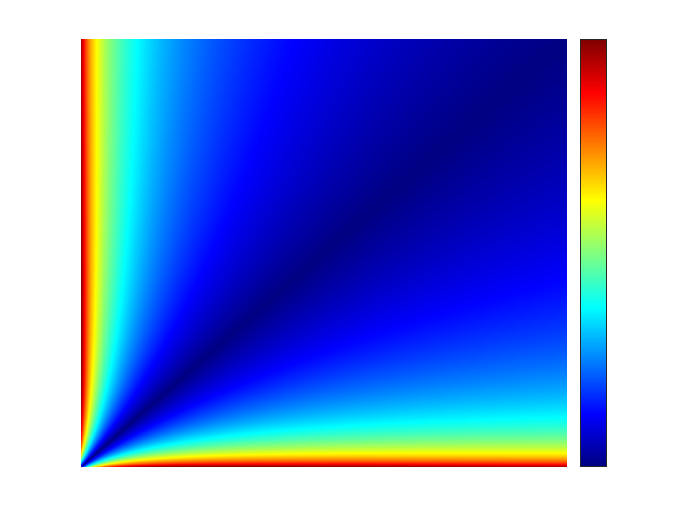
\includegraphics[scale=0.5]{DeltaVHeatmap.png}
    \caption{$\Delta V$ required for a Hohmann transfer between two orbits (created with MATLAB)}\label{fig:Delta V Heatmap}
\end{figure}

In the above figure, $\Delta V$ is represented by the colors, while the axes correspond to the destination and origin orbit radii. It can be seen that the highest $\Delta V$ expenditure occurs when one orbit is very low, while the other is very high.

\bigskip\bigskip
\subsection{Expedited Transfer}

It may at times be the case that the Hohmann Transfer is simply too slow for some applications. If the transfer is from a low orbit to a higher one, then the apoapsis of the transfer orbit can simply be raised higher than the destination orbit. Calculating the $\Delta V$ of such a transfer is elementary, as it requires only application of Equation \eqref{Vis-Viva Equation}. Using Equation \eqref{Time since periapsis}, the transfer time can be evaluated.

\bigskip\bigskip
\subsection{Bi-Elliptic Transfer}

A bi-elliptic transfer is another means of transferring from one circular orbit to another. While a Hohmann transfer takes a spacecraft from one circular orbit to another via a singular transfer orbit, the bi-elliptic transfer utilizes a series of two transfer orbits. First, the spacecraft is put into an orbit much higher than either the source or destination orbit. Then, at the apoapsis of the high transfer orbit, the periapsis is brought to the new orbit.

\begin{figure}[H]
    \centering
    \def\Rone{0.75}
    \def\Rtwo{1.25}
    \def\trAP{4}
    \def\trSMAa{\fpeval{0.5*(\Rone+\trAP)}}
    \def\trSMAb{\fpeval{0.5*(\Rtwo+\trAP)}}
    \def\trEa{\fpeval{(\trAP/\trSMAa) - 1}}
    \def\trEb{\fpeval{(\trAP/\trSMAb) - 1}}
    \def\ctrXa{\fpeval{\Rone-\trSMAa}}
    \def\ctrXb{\fpeval{\Rtwo-\trSMAb}}
    \def\trSmAa{\fpeval{\trSMAa*sqrt(1-(\trEa)^2)}}
    \def\trSmAb{\fpeval{\trSMAb*sqrt(1-(\trEb)^2)}}
    \def\dV{1.25}
    \definecolor{purp}{rgb}{.8,0,.8}
    \definecolor{rurp}{rgb}{.8,0,.4}
    \begin{tikzpicture}[>=latex]
        \draw[thin, dotted, blue] (0,0) ellipse ({\Rone} and {\Rone});
        \draw[blue, thick,>-] (-\Rone,0) arc (180:360:{\Rone} and {\Rone}) node[midway, above] {$r_1$};

        \draw[thin, dotted, purp] (\ctrXa,0) ellipse ({\trSMAa} and {\trSmAa});
        \draw[purp, thick] (\Rone,0) arc (0:180:{\trSMAa} and {\trSmAa}) node[rurp, left] {$r_t$};

        \draw[thin, dotted, red] (\ctrXb,0) ellipse ({\trSMAb} and {\trSmAb});
        \draw[red, thick] (-\trAP,0) arc (180:360:{\trSMAb} and {\trSmAb});

        \draw[thin, dotted,orange] (0,0) ellipse ({\Rtwo} and {\Rtwo});
        \draw[orange, thick,->] (\Rtwo,0) arc (0:180:{\Rtwo} and {\Rtwo}) node[near end, above left] {$r_2$};;

        \filldraw[lightgray] (0,0) circle (2pt);

        \draw[->] (\Rone,0)--+(0,\dV) node[above] {$\Delta v_1$};
        \draw[->] (-\trAP,0)--+(0,-\dV) node[below] {$\Delta v_2$};
        \draw[->] ( \Rtwo,0)--+(0,-\dV) node[below] {$\Delta v_3$};

    \end{tikzpicture}
    \caption{A bi-elliptic transfer from a low orbit to a high orbit (left)}\label{fig:Bielliptic Transfer}
\end{figure}

Figure \ref{fig:Bielliptic Transfer} shows a satellite undergoing a bi-elliptic transfer. It begins in a low orbit (blue) at some radius $r_1$, then performs a burn to enter a high transfer orbit with apoapsis $r_t>r_2$. It then performs a small prograde burn to raise its periapsis to the destination orbit altitude. Finally, at periapsis, it slows down to lower its apoapsis into a circular orbit. Equation \eqref{Vis-Viva Equation} allows this orbit to be analyzed easily much like was done in Section \ref{sec:Hohmann Transfer}.

$a_1=r_1=r_\text{pe,tr}$ is the smaller orbit radius, and $a_2=r_2=r_\text{ap,tr}$ is the larger larger orbit radius. The semi-major axis of the transfer orbits are $a_\text{tr1}=\frac{1}{2}(r_1+r_t)$ and $a_\text{tr2}=\frac{1}{2}(r_2+r_t)$. $v_1$ and $v_2$ refer to the circular orbit velocities in the original and new orbit. Transfer 1 refers to the first transfer orbit (purple in Figure \ref{fig:Bielliptic Transfer}), while transfer 2 refers to the second (red in the same figure).

\begin{align*}
    \Delta V & = \Delta v_1+\Delta v_2+\Delta v_3                                              \\
             & = (v_\text{pe,tr1}-v_1)+(v_\text{ap,tr2}-v_\text{ap,tr1})+(v_2-v_\text{pe,tr2}) \\
\end{align*}

The first burn will always be an accelerative one, while the last will always be declarative. However, the direction of the second burn will depend on whether the origin orbit is higher or lower than the destination orbit. Therefore, the middle burn must have absolute value bars to ensure that its $\Delta V$ contribution is always positive.

\begin{align*}
    \Delta V & = |(v_\text{pe,tr1}-v_1)|+|v_\text{ap,tr2}-v_\text{ap,tr1}|+|v_2-v_\text{pe,tr2}|                                                                   \\
             & = (v_\text{pe,tr1}-v_1)+|v_\text{ap,tr2}-v_\text{ap,tr1}|+(v_\text{pe,tr2}-v_2)                                                                     \\
             & = \left(\sqrt{\frac{2\mu}{r_\text{pe,tr1}}-\frac{\mu}{a_\text{tr}}}-\sqrt{\frac{2\mu}{r_1}-\frac{\mu}{a_1}}\right)                                  \\
             & \phantom{=} +\left|\sqrt{\frac{2\mu}{r_\text{ap,tr2}}-\frac{\mu}{a_\text{tr2}}}-\sqrt{\frac{2\mu}{r_\text{ap,tr1}}-\frac{\mu}{a_\text{tr1}}}\right| \\
             & \phantom{=} +\left(\sqrt{\frac{2\mu}{r_\text{pe,tr2}}-\frac{\mu}{a_\text{tr2}}}-\sqrt{\frac{2\mu}{r_2}-\frac{\mu}{a_2}}\right)                      \\\\
             & = \left(\sqrt{\frac{2\mu}{r_1}-\frac{2\mu}{r_1+r_t}}-\sqrt{\frac{2\mu}{r_1}-\frac{\mu}{r_1}}\right)                                                 \\
             & \phantom{=} +\left|\sqrt{\frac{2\mu}{r_t}-\frac{2\mu}{r_2+r_t}}-\sqrt{\frac{2\mu}{r_t}-\frac{2\mu}{r_1+r_t}}\right|                                 \\
             & \phantom{=} +\left(\sqrt{\frac{2\mu}{r_2}-\frac{2\mu}{r_2+r_t}}-\sqrt{\frac{2\mu}{r_2}-\frac{\mu}{r_2}}\right)                                      \\\\
             & = \left(\sqrt{\frac{2\mu(r_1+r_t)-2\mu r_1}{r_1(r_1+r_t)}}-\sqrt{\frac{\mu}{r_1}}\right)                                                            \\
             & \phantom{=} +\left|\sqrt{\frac{2\mu(r_2+r_t)-2\mu r_t}{r_t(r_2+r_t)}}-\sqrt{\frac{2\mu(r_1+r_t)-2\mu r_t}{r_t(r_1+r_t)}}\right|                     \\
             & \phantom{=} +\left(\sqrt{\frac{2\mu(r_2+r_t)-2\mu r_2}{r_2(r_2+r_t)}}-\sqrt{\frac{\mu}{r_2}}\right)                                                 \\\\
             & = \left(\sqrt{\frac{2\mu r_t}{r_1(r_1+r_t)}}-\sqrt{\frac{\mu}{r_1}}\right)                                                                          \\
             & \phantom{=} +\left|\sqrt{\frac{2\mu r_2}{r_t(r_2+r_t)}}-\sqrt{\frac{2\mu r_1}{r_t(r_1+r_t)}}\right|                                                 \\
             & \phantom{=} +\left(\sqrt{\frac{2\mu r_t}{r_2(r_2+r_t)}}-\sqrt{\frac{\mu}{r_2}}\right)                                                               \\
\end{align*}
\begin{equation}
    \Delta V = \sqrt{\frac{2\mu r_t}{r_1(r_1+r_t)}}+\sqrt{\frac{2\mu r_t}{r_2(r_2+r_t)}}-\sqrt{\frac{\mu}{r_1}}-\sqrt{\frac{\mu}{r_2}}+\left|\sqrt{\frac{2\mu r_2}{r_t(r_2+r_t)}}-\sqrt{\frac{2\mu r_1}{r_t(r_1+r_t)}}\right|
\end{equation}

The time it takes to complete this transfer can be calculated with Equation \eqref{Period Geometric} as the sum of the half-periods of both transfer orbits.
\begin{align*}
    t & =\frac{T_\text{tr1}}{2}+\frac{T_\text{tr2}}{2}                                                             \\
      & =\frac{1}{2}\left(\sqrt{\frac{4\pi^2 a_\text{tr1}^3}{\mu}}+\sqrt{\frac{4\pi^2 a_\text{tr2}^3}{\mu}}\right) \\
      & =\pi\left(\sqrt{\frac{a_\text{tr1}^3}{\mu}}+\sqrt{\frac{a_\text{tr2}^3}{\mu}}\right)                       \\
      & =\pi\left(\sqrt{\frac{(\frac{1}{2}(r_1+r_t))^3}{\mu}}+\sqrt{\frac{(\frac{1}{2}(r_2+r_t))^3}{\mu}}\right)   \\
\end{align*}
\begin{equation}\label{Bielliptic time}
    t_\text{tr}=\pi\left(\sqrt{\frac{(r_1+r_t)^3}{8\mu}}+\sqrt{\frac{(r_2+r_t)^3}{8\mu}}\right)
\end{equation}

\subsubsection{\texorpdfstring{$\Delta V$}{DeltaV} Analysis for Bi-Elliptic Transfers}

Using the same notation as before with $r_2=\alpha r_1$, this equation can be compared to Equation \eqref{Delta V in terms of Alpha Hohmann}. This will allow for comparisons in efficiency.

\begin{align*}
    \Delta V & = \sqrt{\frac{2\mu r_t}{r_1(r_1+r_t)}}+\sqrt{\frac{2\mu r_t}{r_2(r_2+r_t)}}-\sqrt{\frac{\mu}{r_1}}-\sqrt{\frac{\mu}{r_2}}+\left|\sqrt{\frac{2\mu r_2}{r_t(r_2+r_t)}}-\sqrt{\frac{2\mu r_1}{r_t(r_1+r_t)}}\right|                                    \\
             & = \sqrt{\frac{2\mu r_t}{r_1(r_1+r_t)}}+\sqrt{\frac{2\mu r_t}{\alpha r_1(\alpha r_1+r_t)}}-\sqrt{\frac{\mu}{r_1}}-\sqrt{\frac{\mu}{\alpha r_1}}+\left|\sqrt{\frac{2\mu \alpha r_1}{r_t(\alpha r_1+r_t)}}-\sqrt{\frac{2\mu r_1}{r_t(r_1+r_t)}}\right| \\
             & = \sqrt{\frac{\mu}{r_1}}\left(\sqrt{\frac{2r_t}{r_1+r_t}}+\sqrt{\frac{2r_t}{\alpha(\alpha r_1+r_t)}}-\sqrt{\frac{1}{\alpha}}-1\right)+\sqrt{\frac{\mu r_1}{r_t}}\left|\sqrt{\frac{2\alpha}{\alpha r_1+r_t}}-\sqrt{2\frac{1}{r_1+r_t}}\right|
\end{align*}

Now, a new parameter $\beta$ will be defined such that $\beta=\frac{r_t}{r_1}$, or $r_t=\beta$.

\begin{align*}
    \Delta V & = \sqrt{\frac{\mu}{r_1}}\left(\sqrt{\frac{2r_t}{r_1+r_t}}+\sqrt{\frac{2r_t}{\alpha(\alpha r_1+r_t)}}-\sqrt{\frac{1}{\alpha}}-1\right)+\sqrt{\frac{\mu r_1}{r_t}}\left|\sqrt{\frac{2\alpha}{\alpha r_1+r_t}}-\sqrt{2\frac{1}{r_1+r_t}}\right|                                         \\
             & =\sqrt{\frac{\mu}{r_1}}\left(\sqrt{\frac{2\beta r_1}{r_1+\beta r_1}}+\sqrt{\frac{2\beta r_1}{\alpha(\alpha r_1+\beta r_1)}}-\sqrt{\frac{1}{\alpha}}-1\right)+\sqrt{\frac{\mu r_1}{\beta r_1}}\left|\sqrt{\frac{2\alpha}{\alpha r_1+\beta r_1}}-\sqrt{\frac{2}{r_1+\beta r_1}}\right| \\
             & =\sqrt{\frac{\mu}{r_1}}\left(\sqrt{\frac{2\beta}{1+\beta}}+\sqrt{\frac{2\beta}{\alpha(\alpha+\beta)}}-\sqrt{\frac{1}{\alpha}}-1\right)+\sqrt{\frac{\mu}{\beta r_1}}\left|\sqrt{\frac{2\alpha}{\alpha+\beta}}-\sqrt{\frac{2}{1+\beta}}\right|                                         \\
\end{align*}
\begin{equation}\label{Bi-Elliptic DeltaV in terms of alpha, beta, r1}
    \Delta V(\alpha,\beta,r_1) = \sqrt{\frac{\mu}{r_1}}\left(\sqrt{\frac{2\beta}{1+\beta}}+\sqrt{\frac{2\beta}{\alpha(\alpha+\beta)}}-\sqrt{\frac{1}{\alpha}}-1+\left|\sqrt{\frac{2\alpha}{\beta(\alpha+\beta)}}-\sqrt{\frac{2}{\beta(1+\beta)}}\right|\right)
\end{equation}

Because $r_1$ shows up only in the denominator, it is clear that, much like a Hohmann transfer, a bi-elliptic transfer's $\Delta V$ scales with the inverse of the square root of the starting orbit altitude.

\subsection{Comparison of Hohmann and Bi-Elliptic Transfers}

With mathematic analyses completed of both Hohmann and bi-elliptic transfers, the two can be compared to determine when each is more efficient in terms of time and in terms of $\Delta V$ expenditure.

First, transfer times will be analyzed. Equations \eqref{Hohmann time} and \eqref{Bielliptic time} that the transfers have a transfer time of

$$t_\text{Hohmann}=\frac{\pi}{\sqrt{8\mu}}(r_1+r_2)^{3/2}\qquad\text{and}\qquad t_\text{Bi-Elliptic}=\frac{\pi}{\sqrt{8\mu}}\left((r_1+r_t)^{3/2}+(r_2+r_t)^{3/2}\right)$$

It is clear that the bi-elliptic transfer takes substantially longer than the Hohmann transfer, taking at best almost twice as long (as for a Hohmann transfer, only 180 degrees of the orbit must be traversed, whereas the bi-elliptic transfer requires 360 degrees to be traversed). If the bi-elliptic transfer is allowed to approach a bi-parabolic transfer, then the transfer time approaches infinity.

Comparing the $\Delta V$ efficiencies is substantially harder.

Differentiation of \eqref{Bi-Elliptic DeltaV in terms of alpha, beta, r1} with respect to $\beta$ can show the relationship between $\beta$ and $\Delta V$ for a bi-elliptic transfer. Because of how unwieldy this equation is, fewer steps are shown than would be elsewhere. Note that the term inside the absolute value is negative if $\alpha<1$, and positive if $\alpha>1$

%\begin{align*}
%    \frac{\partial\Delta V}{\partial\alpha} &= \frac{\partial}{\partial\alpha}\sqrt{\frac{\mu}{r_1}}\left(\sqrt{\frac{2\beta}{1+\beta}}+\sqrt{\frac{2\beta}{\alpha(\alpha+\beta)}}-\sqrt{\frac{1}{\alpha}}-1+\left|\sqrt{\frac{2\alpha}{\beta(\alpha+\beta)}}-\sqrt{\frac{2}{\beta(1+\beta)}}\right|\right)\\
%    &= \sqrt{\frac{\mu}{r_1}}\left(\frac{\partial}{\partial\alpha}\sqrt{\frac{2\beta}{\alpha(\alpha+\beta)}}-\frac{\partial}{\partial\alpha}\sqrt{\frac{1}{\alpha}}+\frac{\partial}{\partial\alpha}\sqrt{\frac{2\alpha}{\beta(\alpha+\beta)}}\right)\\
%    &= \sqrt{\frac{\mu}{r_1}}\left(\frac{1}{2\alpha^{3/2}}-\sqrt{\frac{\beta}{2\alpha^3(\alpha+\beta)}}\right)\\
%\end{align*}

%Note that $\alpha<\beta$ (and $\beta>1$) at all times, as the transfer apoapsis must be above both the destination and origin orbits. When $\beta>\alpha$, the above expression is always less than zero. This means that a bielliptic transfer, for any given $\beta$, will take less $\Delta V$ for a larger $\alpha$. Recall that the opposite was found for Hohmann transfers, which take \textit{more} $\Delta V$ for a larger transfer. 

\begin{align*}
    \frac{\partial\Delta V}{\partial\beta} & = \frac{\partial}{\partial\beta}\sqrt{\frac{\mu}{r_1}}\left(\sqrt{\frac{2\beta}{1+\beta}}+\sqrt{\frac{2\beta}{\alpha(\alpha+\beta)}}-\sqrt{\frac{1}{\alpha}}-1+\left|\sqrt{\frac{2\alpha}{\beta(\alpha+\beta)}}-\sqrt{\frac{2}{\beta(1+\beta)}}\right|\right)         \\
                                           & = \sqrt{\frac{\mu}{r_1}}\left(\frac{\beta+\operatorname{S}(\alpha)+2\beta\operatorname{S}(\alpha)}{\sqrt{2\beta^3(1+\beta)^3}}+\frac{\alpha\beta-\operatorname{S}(\alpha)\alpha^2-2\alpha\beta\operatorname{S}(\alpha)}{\sqrt{2\alpha\beta^3(\alpha+\beta)^3}}\right) \\
\end{align*}

where $\operatorname{S}(\alpha)$ is defined as
\begin{equation*}
    \operatorname{S}(\alpha)=\begin{cases}
        1  & \alpha>1 \\
        -1 & \alpha<1
    \end{cases}
\end{equation*}

When $\alpha<1$, the derivative never evaluates to zero, and is always positive. This means that when $\alpha<1$, the bi-elliptic transfer becomes more and more inefficient as the transfer apoapsis is raised. In other words, the bi-transfer requires at best the same $\Delta V$ as a Hohmann transfer. Recall that when $\beta=\alpha$, the bi-elliptic transfer is a Hohmann transfer, meaning when $\beta>\alpha$ and $\alpha<1$ the bi-elliptic transfer is less efficient than the simpler Hohmann transfer. The case of $\beta<\alpha$ is also not physically possible, as it does not describe a bi-elliptic transfer. We can therefore discard all $\alpha<1$ for the bi-elliptic transfer analysis, as a Hohmann transfer will be more efficient than the bi-elliptic transfer for this domain. This allows the derivative of \eqref{Bi-Elliptic DeltaV in terms of alpha, beta, r1} to be simplified to

\begin{equation}\label{Bielliptic DV derivative}
    \left(\frac{\partial\Delta V}{\partial\beta}\right)_{\alpha>1} = \sqrt{\frac{\mu}{r_1}}\left(\frac{3\beta+1}{\sqrt{2\beta^3(1+\beta)^3}}-\frac{\alpha}{\sqrt{2\alpha\beta^3(\alpha+\beta)}}\right)
\end{equation}

\eqref{Bi-Elliptic DeltaV in terms of alpha, beta, r1} is always decreasing. In other words, so long as the first derivative is ever negative, the most efficient transfer will occur at the largest $\beta$. Recall that when $\beta=\alpha$, the transfer is a Hohmann transfer. This means $\beta$ is bounded by $\alpha\leq\beta<\infty$.

If the derivative of $\Delta V$ with respect to $\beta$ at $\beta=\alpha$ is negative, it means that increasing $\beta$ will decrease the $\Delta V$, making the transfer at worst just as efficient as a Hohmann transfer. The calculated derivative is always decreasing (the second derivative is always negative), so if there is some $\alpha$ such that $\alpha=\beta$ and the derivative is less than zero, then the $\Delta V$ for a bi-elliptic trajectory will be less than that of a Hohmann transfer for $\beta>\alpha$. Starting at the first $\alpha$ where this occurs, bi-elliptic transfers will always be more efficient than Hohmann transfers.

\begin{align*}
    0                                              & = \left(\frac{\partial\Delta V}{\partial\beta}\right)_{\alpha>1,\alpha=\beta}                                                                      \\
    0                                              & = \sqrt{\frac{\mu}{r_1}}\left(\frac{3\beta+1}{\sqrt{2\beta^3(1+\beta)^3}}-\frac{\alpha}{\sqrt{2\alpha\beta^3(\alpha+\beta)}}\right)_{\alpha=\beta} \\
    0                                              & =\sqrt{\frac{\mu}{r_1}}\left(\frac{3\alpha+1}{\sqrt{2\alpha^3(1+\alpha)^3}}-\frac{\alpha}{\sqrt{2\alpha\alpha^3(\alpha+\alpha)}}\right)            \\
    0                                              & =\frac{3\alpha+1}{\sqrt{2\alpha^3(1+\alpha)^3}}-\frac{\alpha}{\sqrt{2\alpha\alpha^3(\alpha+\alpha)}}                                               \\
    0                                              & =\frac{3\alpha+1}{\sqrt{2\alpha^3(1+\alpha)^3}}-\frac{1}{\sqrt{4\alpha^3}}                                                                         \\
    \frac{3\alpha+1}{\sqrt{2\alpha^3(1+\alpha)^3}} & =\frac{1}{\sqrt{4\alpha^3}}                                                                                                                        \\
    \frac{3\alpha+1}{\sqrt{2\alpha^3(1+\alpha)^3}} & =\frac{2^{-1/2}(1+\alpha)^{3/2}}{\sqrt{2\alpha^3(1+\alpha)^3}}                                                                                     \\
    3\alpha+1                                      & =2^{-1/2}(1+\alpha)^{3/2}                                                                                                                          \\
    9\alpha^2+6\alpha+1                            & =\frac{1}{2}(1+\alpha)^3                                                                                                                           \\
    18\alpha^2+12\alpha+2                          & =1+3\alpha+3\alpha^2+3\alpha^3                                                                                                                     \\
    0                                              & =-\alpha^3+15\alpha^2+9\alpha+1
\end{align*}

This is not factorable. While there is a formula much like the quadratic formula that can solve cubics, it is a very long and unwieldy formula. Instead, this will be solved numerically. The single positive root of this cubic is
$$\alpha=15.58172\dots$$

Beyond this $\alpha$, a bi-elliptic transfer is \textit{always} more efficient than a Hohmann transfer, with the $\Delta V$ requirement decreasing as $\beta$ increases. However, this is not the only time that a bi-elliptic transfer requires less $\Delta V$ than its simpler counterpart.

We will subtract the Hohmann transfer $\Delta V$ from the bi-elliptic transfer one. When this is negative, it means that $\Delta V_\text{Hohmann}>\Delta V_\text{bi-elliptic}$. If this difference is set to zero (and the condition is applied that $\beta>\alpha$), then the $\alpha,\beta$ pairs can be found at which the two transfers are equally efficient. Bi-elliptic will be abbreviated in subscripts as BE, while Hohmann will be abbreviated H.

\begin{align*}
    0 & =\Delta V_\text{BE}-\Delta V _\text{H}                                                                                                                                                                                                               \\
    0 & =\sqrt{\frac{\mu}{r_1}}\left(\sqrt{\frac{2\beta}{1+\beta}}+\sqrt{\frac{2\beta}{\alpha(\alpha+\beta)}}-\sqrt{\frac{1}{\alpha}}-1\right)+\sqrt{\frac{\mu}{r_1}}\left|\sqrt{\frac{2\alpha}{\beta(\alpha+\beta)}}-\sqrt{\frac{2}{\beta(1+\beta)}}\right| \\
      & \phantom{=}-\sqrt{\frac{\mu}{r_1}}\left|\sqrt{\frac{2\alpha}{1+\alpha}}+\sqrt{\frac{1}{\alpha}}-\sqrt{\frac{2}{\alpha(1+\alpha)}}-1\right|                                                                                                           \\\\
    0 & =\left(\sqrt{\frac{2\beta}{1+\beta}}+\sqrt{\frac{2\beta}{\alpha(\alpha+\beta)}}-\sqrt{\frac{1}{\alpha}}-1\right)+\left|\sqrt{\frac{2\alpha}{\beta(\alpha+\beta)}}-\sqrt{\frac{2}{\beta(1+\beta)}}\right|                                             \\
      & \phantom{=}-\left|\sqrt{\frac{2\alpha}{1+\alpha}}+\sqrt{\frac{1}{\alpha}}-\sqrt{\frac{2}{\alpha(1+\alpha)}}-1\right|                                                                                                                                 \\
\end{align*}

Because when $\alpha<1$ the bi-elliptic transfer is less efficient than the Hohmann transfer, $\alpha$ can be assumed to be greater than 1. This means that the absolute values can dissapear, as the expressions inside of them will always be positive.

\begin{align*}
    0 & =\left(\sqrt{\frac{2\beta}{1+\beta}}+\sqrt{\frac{2\beta}{\alpha(\alpha+\beta)}}-\sqrt{\frac{1}{\alpha}}-1\right)+\left(\sqrt{\frac{2\alpha}{\beta(\alpha+\beta)}}-\sqrt{\frac{2}{\beta(1+\beta)}}\right) \\
      & \phantom{=}-\left(\sqrt{\frac{2\alpha}{1+\alpha}}+\sqrt{\frac{1}{\alpha}}-\sqrt{\frac{2}{\alpha(1+\alpha)}}-1\right)
\end{align*}
\begin{equation}\label{Equality for Efficiency}
    \sqrt{\frac{1}{\beta(1+\beta)}}+\sqrt{\frac{\alpha}{1+\alpha}}+\sqrt{\frac{2}{\alpha}}=\sqrt{\frac{\beta}{1+\beta}}+\sqrt{\frac{\beta}{\alpha(\alpha+\beta)}}+\sqrt{\frac{\alpha}{\beta(\alpha+\beta)}}+\sqrt{\frac{1}{\alpha(1+\alpha)}}
\end{equation}

If a bi-elliptic transfer is as efficient as a Hohmann transfer at some $\beta>\alpha$, then it will be more efficient for \textit{all} $\beta$ above that $\alpha$. By allowing $\beta$ to approach infinity, the minimum $\alpha$ can be found such that it satisfies Equation \eqref{Equality for Efficiency}.

\begin{align*}
    \lim_{\beta\rightarrow\infty}\sqrt{\frac{1}{\beta(1+\beta)}}+\sqrt{\frac{\alpha}{1+\alpha}}+\sqrt{\frac{2}{\alpha}} & =\lim_{\beta\rightarrow\infty}\sqrt{\frac{\beta}{1+\beta}}+\lim_{\beta\rightarrow\infty}\sqrt{\frac{\beta}{\alpha(\alpha+\beta)}}+\lim_{\beta\rightarrow\infty}\sqrt{\frac{\alpha}{\beta(\alpha+\beta)}}+\sqrt{\frac{1}{\alpha(1+\alpha)}} \\
    \sqrt{\frac{\alpha}{1+\alpha}}+\sqrt{\frac{2}{\alpha}}                                                              & =1+\sqrt{\frac{1}{\alpha}}+\sqrt{\frac{1}{\alpha(1+\alpha)}}                                                                                                                                                                               \\
    \sqrt{\frac{\alpha^2}{\alpha(1+\alpha)}}+\sqrt{\frac{2(1+\alpha)}{\alpha(1+\alpha)}}                                & =\sqrt{\frac{\alpha(1+\alpha)}{\alpha(1+\alpha)}}+\sqrt{\frac{1+\alpha}{\alpha(1+\alpha)}}+\sqrt{\frac{1}{\alpha(1+\alpha)}}                                                                                                               \\
    0                                                                                                                   & =\alpha+\sqrt{2(\alpha+1)}-\sqrt{\alpha(\alpha+1)}-\sqrt{\alpha+1}-1
\end{align*}

This is unfortunately not analytically solvable, but it can be solved with numerical methods. It yields

$$\alpha\approx11.93876$$

At all $\alpha<11.93876$, a Hohmann transfer is more efficient. At all $\alpha>15.58172$, a bi-elliptic transfer is always more efficient. Between these two $\alpha$ values, the choice of $\beta$ determines which is more efficient. Of course, the transfer time approaches infinity as $\beta$ approaches infinity, which is required for the bi-elliptic transfer to be more efficient than the Hohmann transfer as $\alpha\rightarrow11.93876$.

\bigskip\bigskip
\subsection{Combined Manuever}

Any single-burn maneuver can be done most efficiently by burning such that $\Delta V$ takes the velocity from some original velocity $\vv{v}_1$ to some desired velocity $\vv{v}_2$. In all probability, the velocity vector of a satellite will be known by measurement. If instead the geometric parameters of the orbit are known, Equations \eqref{Vis-Viva Equation} and \eqref{Flight Path Angle} can be used to determine the velocity vector in the plane of the orbit. The desired velocity vector can be found with the same equations, and using basic trigonometry changes in inclination can be accounted for as well. For maneuvers in which the location of the ascending and descending nodes changes, some geometry must be applied. For any maneuver where the only change in inclination occurs at the ascending or descending node, the calculation is relatively simple. We will assume that the original velocity $v_1$ and the new velocity $v_2$ are both known, the change in flight path angle $\Delta \phi$ is known, and the angle between the old and new orbital planes $\Delta j$ is known. Using this, the total $\Delta V$ required can be calculated. The law of cosines can be used to simplify this calculation, however for ease of following it will not be used.

\begin{align*}
    \Delta V & = |\vv{v}_2-\vv{v}_1|                                                                                                                                           \\
             & = |v_2(\cos(\Delta \phi)\cos(\Delta j)\hat{m}_v+\sin(\Delta \phi)\cos(\Delta j)\hat{m}_r+\sin(\Delta j)\hat{m}_n)-v_1\hat{m}_v|                                 \\
             & = |(v_2\cos(\Delta \phi)\cos(\Delta j)-v_1)\hat{m}_v+v_2\sin(\Delta \phi)\cos(\Delta j)\hat{m}_r+v_2\sin(\Delta j)\hat{m}_n|                                    \\
             & = \sqrt{(v_2\cos(\Delta \phi)\cos(\Delta j)-v_1)^2+(v_2\sin(\Delta \phi)\cos(\Delta j))^2+(v_2\sin(\Delta j))^2}                                                \\
             & = \sqrt{v_2^2\cos^2(\Delta \phi)\cos^2(\Delta j)+v_1^2-2v_1v_2\cos(\Delta \phi)\cos(\Delta j)+v_2^2\sin^2(\Delta \phi)\cos^2(\Delta j)^2+v_2^2\sin^2(\Delta j)} \\
             & = \sqrt{v_1^2+v_2^2\cos^2(\Delta \phi)\cos^2(\Delta j)+v_2^2\sin^2(\Delta \phi)\cos^2(\Delta j)+v_2^2\sin^2(\Delta j)-2v_1v_2\cos(\Delta \phi)\cos(\Delta j)}   \\
             & = \sqrt{v_1^2+v_2^2\cos^2(\Delta j)(\cos^2(\Delta \phi)+\sin^2(\Delta \phi))+v_2^2\sin^2(\Delta j)-2v_1v_2\cos(\Delta \phi)\cos(\Delta j)}                      \\
             & = \sqrt{v_1^2+v_2^2\cos^2(\Delta j)+v_2^2\sin^2(\Delta j)-2v_1v_2\cos(\Delta \phi)\cos(\Delta j)}                                                               \\
             & = \sqrt{v_1^2+v_2^2(\cos^2(\Delta j)+\sin^2(\Delta j))-2v_1v_2\cos(\Delta \phi)\cos(\Delta j)}                                                                  \\
             & = \sqrt{v_1^2+v_2^2-2v_1v_2\cos(\Delta \phi)\cos(\Delta j)}                                                                                                     \\
\end{align*}

For any manuever where the beginning and end velocity vectors are known, the required $\Delta V$ is

\begin{equation}
    \Delta V = \sqrt{v_1^2+v_2^2-2v_1v_2\cos(\Delta \phi)\cos(\Delta j)}
\end{equation}

If instead the angle $\varPhi$ between the vectors is known, this simplifies to

\begin{equation}
    \Delta V = \sqrt{v_1^2+v_2^2-2v_1v_2\cos(\varPhi)}
\end{equation}

\bigskip\bigskip
\subsection{Conclusion}

\bigskip
To change the inclination of an orbit, a normal burn should be done at either the ascending or descending node. The $\Delta V$ required to change the inclination by a given amount is
$$\Delta V=2\sin\left(\frac{\Delta i}{2}\right)$$

\bigskip
To transfer between two circular orbits, the most simple trajectory is a Hohmann transfer, in which a satellite first enters a transfer orbit that is tangent to both the destination and origin orbits, and then circularizes at the destination orbit. If $\alpha$ describes the ratio of source orbit to destination orbit and $r_1$ is the origin orbit's radius, the $\Delta V$ required for a Hohmann transfer is
$$\Delta V_\text{Hohmann} = \sqrt{\frac{\mu}{r_1}}\left|\sqrt{\frac{2\alpha}{1+\alpha}}+\sqrt{\frac{1}{\alpha}}-\sqrt{\frac{2}{\alpha(1+\alpha)}}-1\right|$$

Time time it takes for a Hohmann transfer is
$$t_\text{Hohmann}=\pi\sqrt{\frac{(r_1+r_2)^3}{8\mu}}$$

\bigskip
A bi-elliptic transfer, much like a Hohmann transfer, transfers between two orbits with a ratio $\alpha=r_2/r_1$. A bi-elliptic transfer takes three burns, instead of the two that are needed for a Hohmann transfer. In a bi-elliptic transfer, the transfer orbit has an apoapsis above both the origin and destination orbits. If $\beta$ describes the ratio of this apoapsis to the origin orbit radius, then the $\Delta V$ required for a bi-elliptic transfer is
$$\Delta V_\text{bi-elliptic} = \sqrt{\frac{\mu}{r_1}}\left(\sqrt{\frac{2\beta}{1+\beta}}+\sqrt{\frac{2\beta}{\alpha(\alpha+\beta)}}-\sqrt{\frac{1}{\alpha}}-1+\left|\sqrt{\frac{2\alpha}{\beta(\alpha+\beta)}}-\sqrt{\frac{2}{\beta(1+\beta)}}\right|\right)$$

with a longer transfer time of
$$t_\text{bi-elliptic}=\pi\left(\sqrt{\frac{(r_1+r_t)^3}{8\mu}}+\sqrt{\frac{(r_2+r_t)^3}{8\mu}}\right)$$

For all $\alpha<11.93876$, a Hohmann transfer is always more efficient than a bi-elliptic transfer. For all $\alpha>15.58172$, a bi-elliptic transfer is more efficient. For all $\alpha$ between these values, there exists a $\beta$ above which the bi-elliptic transfer is more efficient and below which the Hohmann transfer is more efficient.

\bigskip

For complex single-burn maneuvers in which both the beginning velocity vector and desired velocity vector are known, the $\Delta V$ required to complete the maneuver is
$$\Delta V = \sqrt{v_1^2+v_2^2-2v_1v_2\cos(\Delta \phi)\cos(\Delta j)}$$


\end{document}